\documentclass[11pt]{article}
\usepackage[margin=1in]{geometry}
\usepackage{amsmath,amssymb,amsthm,booktabs,longtable,array,pdflscape,xcolor}
\usepackage{xr-hyper}
\usepackage{hyperref}
\usepackage{flafter}
\usepackage{placeins}
\usepackage{tikz}
\usetikzlibrary{arrows.meta,positioning,fit,backgrounds}
\definecolor{darkblue}{rgb}{0.0, 0.0, 0.55}
\usepackage[T1]{fontenc}
\externaldocument[P-]{paper}
\newcommand{\pref}[1]{\ref*{P-#1}}
\newcommand{\peqref}[1]{(\ref*{P-#1})}
\newcommand{\lean}[1]{\begingroup\def\_{\textunderscore\allowbreak}\texttt{\small #1}\endgroup}
\newcommand{\artifactlink}{\href{https://github.com/lintingyee-del/fixed-price-bilateral-trade}{artifact repository}}
\title{Machine-Checked Proofs for \emph{The Exact Welfare Guarantee of Fixed-Price Bilateral Trade}\\
\large Formalization Supplement}
\author{}
\date{}

\begin{document}
\emergencystretch=2em
\maketitle

\section{What we checked}

We formalized the paper's results in Lean~4 against Mathlib. The
accompanying \artifactlink{} contains the Lean sources, the statement
manifest and its checker, and the exact and interval-arithmetic
certificates for the computer-assisted statements.

The development contains 130 Lean source files and 1,701 theorem or lemma
declarations in the library \lean{FixedPrice}. A full build completes 8,605
jobs with no errors. Source scans contain no \lean{sorry}, no custom axiom,
and no \lean{native\_decide}; every credentialed statement rests only on
Lean's standard foundational axioms \lean{propext}, \lean{Classical.choice},
and \lean{Quot.sound}. The manifest has 101 non-assumption nodes, of which
44 carry a Lean credential. Each of the five lettered theorems and both
lettered corollaries has a Lean counterpart among them.

The principal single-unit bounds and optimization results are
formalized with no hypothesis beyond the printed ones. The statement
comparison in Section~\ref{s:gaps} identifies clauses not exported by
the Lean declarations. Lean proves Theorem~\pref{thm:exact}, including the
uniqueness of the root $C_*$, the strict inequality for every pair, and
the bounded pairs that approach $\beta_*$. It proves the frontier of
Theorem~\pref{thm:frontier} with its conditional form and conjugate
duality, the four asymptotic equivalences of
Corollary~\pref{cor:asymptotics}, Theorem~\pref{thm:calibration} with the
almost-everywhere uniqueness of the maximizing control, and the
dominant-strategy ceiling of Corollary~\pref{cor:dsic} with the price
representation of Proposition~\pref{lem:representation}.
Theorem~\pref{thm:two-separation} is proved by exact evaluation of its two
finite instances in the Lean kernel.

The two-unit analysis beyond Theorem~\pref{thm:two-separation} is
formalized conditionally. Theorem~\pref{thm:two-pricing}, its finite-node
recurrence in Appendix~\pref{app:two-recurrence},
Proposition~\pref{prop:2fam-optimum}, and six of the seven lemmas behind it
assume, as named hypotheses, scalar facts, identities and enclosures that
exact, interval or SMT arithmetic already certifies
(Section~\ref{s:conditional}). The shape lemma,
Lemma~\pref{lem:2fam-shape}, needs no such hypothesis.

The manifest records the remaining statements one by one.
Proposition~\pref{prop:two-tail}, Proposition~\pref{prop:2fam-separate-responses},
and the reduction of Conjecture~\pref{conj:two-exact} to the budget bound
\peqref{eq:two-open-budget} keep their analytic proofs, and the conjecture
itself is open. Lemma~\pref{lem:reference} is formalized in the parts that
the proof of Theorem~\pref{thm:calibration} uses, without its monotone
parametrization of the endpoints. From the paper's
Section~\pref{sec:model}, the arctangent form of $\mathcal I$, the existence of a best price, and the
fact that randomized prices do no better are not stated in Lean; neither is
the two-step formula \peqref{eq:9} behind the nonconcavity example of
Appendix~\pref{app:nonconcavity}, whose gap $11/1728$ is checked in exact
arithmetic. Decimal values, among them $\beta_*\approx0.73802$ and the
comparison $0.7290804<0.738024<\beta_*$ in
Theorem~\pref{thm:two-separation}, come from interval arithmetic outside
Lean.

\paragraph{What a credential is attached to.}
A credential is issued against a pair: the statement of a node, and the set
of premises it stands on. The manifest stores a fingerprint of that pair,
and the checker recomputes it. Changing a statement or rewiring a premise
therefore invalidates the credential. This check compares the stored statement and premise set with their
recorded fingerprint. It does not read the TeX or compare its meaning with
a Lean type; that correspondence requires the separate review described
in Section~\ref{s:table}.

\section{The manifest as a graph}
\label{s:graph}

The manifest is a directed graph. One vertex represents each statement it
tracks, and an edge from $P$ to $Q$ records that the proof of $Q$ uses $P$.
At this revision it has 103 vertices and 164 edges. Thirty-five vertices
record the paper itself: 2 assumptions, 4 definitions, and 29 statements.
Twenty-four record scalar facts certified by exact, interval or SMT
arithmetic, and 44 record Lean renderings of printed results. Forty-one
vertices are sources and 31 are sinks. The graph is acyclic, and a manifest
containing a cycle fails to load.

\paragraph{A credential is issued against a vertex together with its in-edges.}
We fingerprint the pair consisting of a node's statement and its sorted
premise set, so the record for Lemma~\pref{lem:gaps} reads

\begin{quote}
\lean{sha256:2c80e5b31004 = sha256(<statement of P\_gaps> |}\\
\lean{P\_energy,P\_preliminaries,P\_reference)}
\end{quote}

where the statement is the text of the lemma as printed. Editing the
statement moves the fingerprint, and so does adding a premise, dropping
one, or rerouting an edge. The next \lean{check} then refuses the
credential. Figure~\ref{fig:cone} draws the in-neighbourhood that
Lemma~\pref{lem:gaps} is fingerprinted against.

\begin{figure}[tb]
\centering
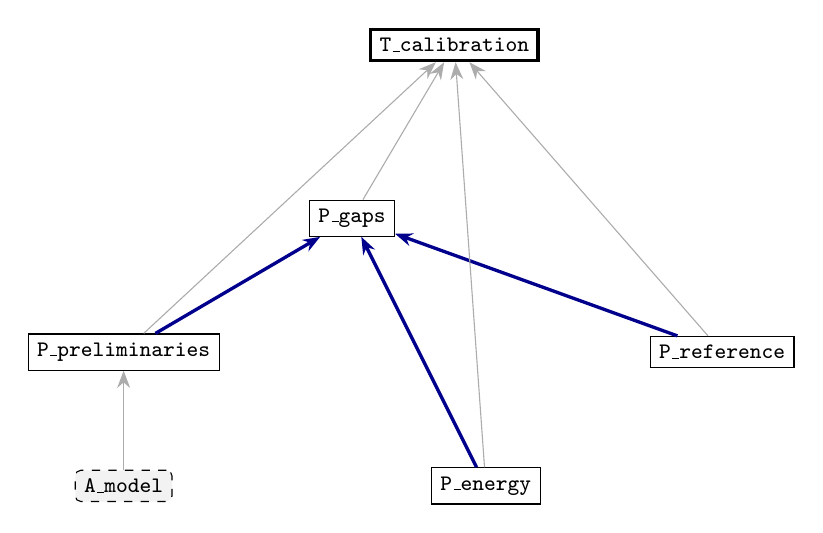
\begin{tikzpicture}[
  >={Stealth[length=2.2mm]},
  assum/.style={draw,dashed,rounded corners=2pt,fill=black!5,
                font=\footnotesize\ttfamily,inner sep=3.2pt},
  stmt/.style={draw,font=\footnotesize\ttfamily,inner sep=3.2pt},
  thm/.style={draw,very thick,font=\footnotesize\ttfamily,inner sep=3.2pt},
  dep/.style={->,gray!65},
  key/.style={->,very thick,darkblue}
]
\node[assum] (mod) at (0,0)     {A\_model};
\node[stmt]  (pre) at (0,1.7)   {P\_preliminaries};
\node[stmt]  (ene) at (4.6,0)   {P\_energy};
\node[stmt]  (ref) at (7.6,1.7) {P\_reference};
\node[stmt]  (gap) at (2.9,3.4) {P\_gaps};
\node[thm]   (cal) at (4.2,5.6) {T\_calibration};

\draw[key] (pre) -- (gap);
\draw[key] (ene) -- (gap);
\draw[key] (ref) -- (gap);

\draw[dep] (mod) -- (pre);
\draw[dep] (pre) -- (cal);
\draw[dep] (ene) -- (cal);
\draw[dep] (ref) -- (cal);
\draw[dep] (gap) -- (cal);
\end{tikzpicture}
\caption{The dependency cone of Theorem~\pref{thm:calibration}, drawn from
the manifest: six vertices and eight edges. Edges run from premise to
conclusion, so reading upward follows the paper's argument. The dashed box
is an assumption, which carries no credential by construction, and the
thick box is a theorem. The three \textcolor{darkblue}{\textbf{bold edges}}
are the in-neighbourhood \texttt{P\_gaps} is fingerprinted against. Cones
elsewhere in the manifest run much wider, with 28 vertices downstream of
\texttt{A\_two\_model}.}
\label{fig:cone}
\end{figure}

\paragraph{The two reachability queries.}
Downstream, \lean{blast <node>} returns the descendant closure: what else
falls if this statement falls. The two-unit model
\texttt{A\_two\_model} reaches 28 of the 103 vertices, and the calculus of
the single-unit contact branch, \texttt{L\_lean\_branch\_calculus}, reaches
18. Upstream, \lean{audit <node>} returns the ancestor closure together with
the credential state of every vertex in it, so we can see whether the route
to a theorem passes through anything uncertified. The longest chain in the
graph runs 10 edges, from \texttt{L\_lean\_branch\_calculus} through the
local and global contact branch, the bound and the uniqueness clause of
Theorem~\pref{thm:calibration}, the strict inequality and the finite-tail
estimate, and Theorem~\pref{thm:exact} itself, to
Corollary~\pref{cor:dsic}. At that length inspection stops being reliable
and the closure does the work.

\paragraph{The manifest graph and Lean's.}
Lean keeps a dependency graph of its own, whose vertices are declarations,
and enforces it directly: a Lean proof cannot use a lemma that is not
there. The verification work happens there, and the manifest does none of
it. The manifest records which printed statements carry which evidence, on
which premises. Each Lean credential sits on a vertex of its own beside the
paper's vertex: the paper's vertex keeps the in-edges of the printed proof,
and the Lean vertex those of the formal proof, certified facts included.
The printed proof of Theorem~\pref{thm:two-pricing} uses its scalar facts as
steps, while its Lean vertex lists their certificates as premises, so a
change to a certificate shows up in the audit of the Lean result. For the
single-unit results the Lean vertices mirror the decomposition of the Lean
development.

Degrees carry a different kind of information. The checker's
\lean{status} report flags vertices with no descendants and four or more
ancestors, currently 12 of them, as costly but load-bearing for nothing.
This is a proportionality diagnostic, not a correctness test: a corollary
can be sound and still require a deep chain that supports no later result.

\FloatBarrier
\section{Verification Layers}

The claims call for different verification methods.

\paragraph{Deductive claims, which we checked in Lean.}
Theorems, propositions and lemmas assert implications from stated premises.
Of the 29 paper statements in the manifest, 25 have a Lean counterpart,
including 9 conditional on certified facts. Coverage ranges from full
statements to selected components, as specified below.
Section~\ref{s:table} pairs each with its declarations, and
Section~\ref{s:outside} accounts for the other 4.

\paragraph{Finite computations, which we checked in exact and interval arithmetic.}
Several claims concern specific numbers: the decimal enclosure of
$\beta_*$ and the data of the finite-tail pairs, the lower bound $73/100$ on
the two affine boundary families of the curve family, the stationary point
of that family and its physical margins, and the rational polygon of
Lemma~\pref{lem:2fam-witness}. Exact rational arithmetic, Bernstein
expansion and Arb ball arithmetic check them outside Lean
(Section~\ref{s:certificates}). The two instances of
Theorem~\pref{thm:two-separation} are checked twice: by exact rational
arithmetic in the replay script, and inside the Lean kernel by
\lean{decide +kernel} on the stored integers.

\paragraph{Symbolic and scalar facts.}
Identities that expand to zero and first-order inequalities over the reals
are certified by exact SymPy expansion, or by the SMT solvers z3 and cvc5
separately. Where a Lean proof needs such a fact, the fact enters as a
hypothesis (Section~\ref{s:conditional}).

\paragraph{Interpretive statements.}
Several passages make no mathematical claim, among them the reading of the
frontier in the paper's Section~\pref{sec:frontier} and the comparison with
related mechanisms in its Section~\pref{sec:related}. The numerical evidence offered for
Conjecture~\pref{conj:two-exact} in Section~\pref{sec:two-open} is
floating-point exploration and carries no credential.

\section{The certificates outside Lean}
\label{s:certificates}

The directory \lean{supplement/} contains the finite instances of
Theorem~\pref{thm:two-separation}, the interval data of the two-unit
family, and the replay script \lean{verify.py}. The script reads every
certificate from its data file and re-evaluates it without search: exact
rationals for the instances, the Bernstein trees on the affine boundary
families, and Arb balls for $\beta_*$, the finite-tail pairs, both covers of
the stationary branch, and the root strip. For the files of identities and
sign enclosures it confirms the recorded zero residuals and signs rather
than re-deriving them. Running it from that directory,

\begin{quote}
\lean{python verify.py}
\end{quote}

prints one line per check, among them

\begin{quote}
\lean{PASS\ \ beta\_*: 0.73802433573 < beta\_* < 0.73802433574}\\
\lean{PASS\ \ general instance: ratio < 0.7290804\ \ \ ratio = 0.7290803900752}\\
\lean{PASS\ \ stationary\_uniform\_cover.json: leaves tile t in [1/5, 421/1000]}
\end{quote}

and ends with \lean{37 checks, 0 failed}. The scalar facts carried by the
hypothesis structures of Section~\ref{s:conditional} were checked by exact
SymPy expansion or by both z3 and cvc5. The repository includes the checking scripts, their receipts, and the
shared Python helpers they import. Every Lean field names the check it
relies on.

\section{Certified facts as Lean hypotheses}
\label{s:conditional}

For the two-unit results we followed one rule: a fact that an exact,
interval or SMT certificate already establishes is not proved again in
Lean. It enters the Lean statement as a field of a hypothesis structure.
Each field states the certified formula in the notation of the Lean
definitions, and its documentation names the paper passage that uses it and
the certificate record that establishes it, and says what that certificate
checks and no more. There are four structures.

\begin{itemize}
\item \lean{PricingScalarCertificates} (12 fields), in
\lean{TwoUnit/Pricing/Defs.lean}: four identities and Farkas certificates
for the price constraints, checked by exact expansion, and eight scalar
inequalities, among them the contraction factor $\bar b/(1+\bar b)$ of the
kernel and four pointwise facts about rounded buyers, each checked by both
z3 and cvc5.
\item \lean{NodeScalarCertificates} (4 fields), in
\lean{TwoUnit/Pricing/FiniteNodes.lean}: a backward step of the node
recurrence is the least value above its three bounds and preserves order,
kernel summands compare termwise (z3 and cvc5), and the three-way maximum
is convex (exact, 27 branch certificates).
\item \lean{FamilyNumerics} (10 fields), in
\lean{TwoUnit/Family/Certificates.lean}: the value of the small-mass bound
\peqref{eq:2fam-small-mass} at $1/32$, the bound $73/100$ on the two affine
boundary families, seven rational constants of the proof of
Lemma~\pref{lem:2fam-domain}, the existence, uniqueness and physical
margins of the stationary point over the whole interval of trial ratios,
its comparison sign at the lower trial ratio, and the rational polygon of
Lemma~\pref{lem:2fam-witness}.
\item \lean{FamilyIdentities} (52 fields), in the same file: closed-form
identities of the curve family, among them the quadratures, the first
integral of the Euler equation, the contact densities, the reconstruction
formulas, the stationarity reductions, and the price-region algebra of the
realization lemma, each an exact symbolic residual or a check by both
solvers.
\end{itemize}

Theorem~\pref{thm:two-pricing} assumes \lean{PricingScalarCertificates}, and
the finite-node recurrence assumes both pricing structures.
Lemma~\pref{lem:2fam-witness} assumes \lean{FamilyNumerics},
Lemma~\pref{lem:2fam-realization} assumes \lean{FamilyIdentities}, and
Proposition~\pref{prop:2fam-optimum} with
Lemmas~\pref{lem:2fam-compact} and~\pref{lem:2fam-boundary}--\pref{lem:2fam-cover}
assume both family structures. A conditional credential therefore reads:
the printed statement follows in Lean from these fields. The fields are
arguments of the theorem, such as \lean{cert : PricingScalarCertificates},
not axioms, so \lean{\#print axioms} does not list them and \lean{\#check}
does.

The two interval covers of the stationary branch are certified only under
the premise that the algebraic residual increases in $p_{\mathrm f}$. The
four fields that rest on them carry that premise explicitly, and Lean
discharges it from the second claim of Lemma~\pref{lem:2fam-domain}, which
it proves from certified constants and identities.

\section{How to rerun the checks}

The toolchain is pinned: Lean \lean{leanprover/lean4:v4.30.0} and Mathlib at
revision \lean{c5ea00351c28} (tag \lean{v4.30.0}), the only dependency. From
the project directory
\lean{research\_ideas/probes/fixed\_price/lean/} of the repository,
after \lean{lake exe cache get} has fetched Mathlib's compiled files:

\begin{quote}
\lean{lake build}
\end{quote}

A clean build of the credentialed development exits zero. It includes the
kernel evaluation of the two instances of
Theorem~\pref{thm:two-separation}, which takes about four minutes. A single
file typechecks on its own with \lean{lake env lean <file>}, writing
nothing.

A successful build permits incomplete proofs and additional axioms, so
we check axiom dependencies separately. In a file importing
\lean{FixedPrice}, the command

\begin{quote}
\lean{\#print axioms FixedPrice.theoremA}
\end{quote}

should print exactly \lean{[propext, Classical.choice, Quot.sound]}. If
\lean{sorryAx} shows up in that list, some proof in the dependency closure
is incomplete; any other name means a custom axiom was admitted somewhere.
The same holds for every conditional result, whose certified facts sit in
its type instead:

\begin{quote}
\lean{\#check @FixedPrice.TwoUnit.Family.prop\_2fam\_optimum}
\end{quote}

prints \lean{FamilyNumerics $\to$ FamilyIdentities $\to$ OptimumStatement}.
We also check that the manifest is internally consistent. From the
repository root, the command

\begin{quote}
\lean{python proof\_factgraph/factgraph.py}\\
\lean{research\_ideas/probes/fixed\_price/manuscript/factgraph.toml check}
\end{quote}

recomputes every fingerprint, reports any credential whose statement or
premise set has moved since it was issued, and rejects dangling references
and cycles in the dependency graph. At this revision it prints
\lean{ok: 103 nodes, no dangling refs, no cycles}.

\section{Paper statements and their Lean counterparts}
\label{s:table}

The table pairs each numbered result with its available Lean counterpart,
in the order of the paper. Where a row is only partial or conditional
coverage, the row says so explicitly; the manifest, rather than this table,
decides whether the complete paper node carries a credential. File paths
are relative to \lean{lean/FixedPrice/}, and names relative to the
namespace of their file.

The repository also includes \lean{statement\_correspondence.py} and
its generated TeX/Lean excerpts. The script extracts the table's labels,
locates their declarations, and expands the named statement abbreviations
and certificate structures. It detects missing names and incorrect file
locations. Agreement of quantifiers, assumptions, definitions and equality
cases still requires a semantic review; the script issues no equivalence
certificate. The scope differences below remain part of that review.

The repository also includes \lean{statement\_correspondence.py} and
its generated TeX/Lean excerpts. The script extracts the table's labels,
locates their declarations, and expands the named statement abbreviations
and certificate structures. It detects missing names and incorrect file
locations. Agreement of quantifiers, assumptions, definitions and equality
cases still requires a semantic review; the script issues no equivalence
certificate. The scope differences below remain part of that review.

\begin{landscape}
\scriptsize
\begin{longtable}{@{}>{\raggedright\arraybackslash}p{0.14\linewidth}>{\raggedright\arraybackslash}p{0.50\linewidth}>{\raggedright\arraybackslash}p{0.31\linewidth}@{}}
\toprule
Paper statement & Lean declaration & File \\
\midrule
\endhead
Sec.~\pref{sec:model}, scalar curve & \peqref{eq:7} and the monotonicity of $S$ and $\tau$: \lean{hasDerivAt\_optimalValue}, \lean{optimalValue\_strictAntiOn}, \lean{initialState\_strictMonoOn}; limits \peqref{eq:8}: \lean{optimalValue\_tendsto\_left} and its three companions; $S$ onto $(1,\infty)$: \lean{existsUnique\_optimalValue\_eq}; the arctangent form of $\mathcal I$, the best price and the randomization clause outside Lean & \lean{ScalarCurve.lean}, \lean{FrontierCurve.lean} \\
Thm.~\pref{thm:exact}\newline\texttt{thm:exact} & \lean{theoremA}: every pair above $\beta_*$, bounded pairs below $\beta_*+\varepsilon$, and $\beta_*$ as greatest lower bound; the root $C_*$: \lean{existsUnique\_root}; the decimal value of $\beta_*$ outside Lean & \lean{TheoremA.lean}, \lean{Strict.lean}, \lean{ScalarCurve.lean} \\
Thm.~\pref{thm:frontier}\newline\texttt{thm:frontier} & \lean{theoremB\_affine}, \lean{frontierDelta\_eq} for \peqref{eq:47}; boundedness of the refuting and approaching pairs is not in the exported types; \lean{frontierDelta\_strictMonoOn}, \lean{frontierDelta\_strictConvexOn}, \lean{frontierDelta\_deriv\_image}; \lean{kappaOf\_strictMonoOn}, \lean{existsUnique\_kappaOf\_eq} for \peqref{eq:51}; \lean{theoremB\_conditional}, \lean{condRatio\_eq} for \peqref{eq:52}; \lean{theoremB\_conjugate} for \peqref{eq:53} & \lean{FrontierAffine.lean}, \lean{FrontierConvex.lean}, \lean{FrontierCurve.lean}, \lean{FrontierConditional.lean} \\
Cor.~\pref{cor:asymptotics}\newline\texttt{cor:asymptotics} & \lean{frontierDelta\_isEquivalent\_zero}, \lean{frontierDelta\_isEquivalent\_one}, \lean{condRatio\_isEquivalent\_zero}, \lean{condRatio\_isEquivalent\_top} & \lean{Asymptotics.lean} \\
Lem.~\pref{lem:energy}\newline\texttt{lem:energy} & \lean{reciprocalState\_hasDerivAt\_at\_tailTime}, \lean{reciprocalState\_bounds}, \lean{reciprocalState\_line\_obstacle}, \lean{reciprocal\_energy\_identity\_extended}; original-time form \lean{objective\_originalTime\_identity} & \lean{Reciprocal.lean}, \lean{Controls.lean} \\
Lem.~\pref{lem:reference}\newline\texttt{lem:reference} & component coverage only: contact branch \lean{local\_contact\_branch\_exists}, \lean{hasBranchRoot\_of\_le}, \lean{hasBranchRoot\_eventually}; every endpoint reached, \lean{exists\_branch\_point}; \peqref{eq:18} by \lean{IsBranchRoot.contact\_line}, \lean{IsBranchRoot.contact\_arc}, \lean{IsBranchRoot.contact\_cap}; energy \lean{IsBranchRoot.logEnergy\_refLog}; the parametrization by $\bar C(d)$, the monotone bijection $C\mapsto x(C)$ and the $C^1$ regularity of $P_x$ not stated & \lean{BranchRegularity.lean}, \lean{GlobalBranch.lean}, \lean{Coverage.lean}, \lean{ReferenceCurve.lean}, \lean{ReferenceEnergy.lean} \\
Lem.~\pref{lem:gaps}\newline\texttt{lem:gaps} & (G1): \lean{logEnergy\_gap\_identity\_weight}, \lean{logEnergy\_le\_of\_weight\_calibration}, \lean{eqOn\_zero\_of\_weight\_calibration}; (G2): \lean{hasDerivAt\_endpointValue}, \lean{physicalEndpoint\_calibration}, \lean{endpointValue\_branch\_le} & \lean{CalibrationAE.lean}, \lean{EndpointDerivative.lean}, \lean{PhysicalBranch.lean}, \lean{GlobalBranch.lean} \\
Thm.~\pref{thm:calibration}\newline\texttt{thm:calibration} & \lean{theoremC}: bound, attainment by \peqref{eq:31}, and uniqueness almost everywhere; components \lean{objective\_le\_optimalValue}, \lean{maximizingControl\_attains}, \lean{objective\_eq\_optimalValue\_iff}; inputs to \peqref{eq:29} for $C>0$; its $C=0$ endpoint identity not stated & \lean{TheoremC.lean}, \lean{UpperBound.lean}, \lean{Attainment.lean}, \lean{Uniqueness.lean} \\
Prop.~\pref{prop:nonexponential}\newline\texttt{prop:nonexponential} & \lean{proposition\_nonexponential}, without the condition $h'>0$ & \lean{NoExponential.lean} \\
Lem.~\pref{lem:pricing}\newline\texttt{lem:pricing} & \lean{exists\_price\_of\_variational\_bound}, for every $\beta\ge0$ & \lean{PricingLemma.lean} \\
Lem.~\pref{lem:hard}\newline\texttt{lem:hard} & \lean{HardPairData.sellerMean\_eq}, \lean{HardPairData.gainsFromTrade\_eq}; $\Gamma_{\max,\eta}$ and \peqref{eq:41} as upper bounds: \lean{HardPairData.gain\_le}, \lean{HardPairData.welfare\_gap\_le} & \lean{HardBuyer.lean}, \lean{HardSeller.lean}, \lean{HardPair.lean} \\
Lem.~\pref{lem:smoothing}\newline\texttt{lem:smoothing} & \lean{lemma\_smoothing}, in $\varepsilon$--$\delta$ form, without the full-support clause & \lean{Smoothing.lean} \\
Prop.~\pref{lem:representation}\newline\texttt{lem:representation} & \lean{DSICOn.representation}, \lean{DSICOn.mechWelfare\_le}, for a class containing the paper's & \lean{Mechanism.lean}, \lean{MechanismWelfare.lean} \\
Cor.~\pref{cor:dsic}\newline\texttt{cor:dsic} & \lean{corollary\_dsic}, with \lean{dsic\_guarantee} and \lean{dsic\_ceiling}, for a class containing the paper's & \lean{CorollaryDSIC.lean}, \lean{DSICClass.lean} \\
\midrule
Thm.~\pref{thm:two-separation}\newline\texttt{thm:two-separation} & \lean{TwoUnit.theoremD\_general}, \lean{TwoUnit.theoremD\_symmetric}, by kernel evaluation; the comparison with $\beta_*$ uses the interval enclosure outside Lean & \lean{TwoUnit/TheoremD.lean}, \lean{TwoUnit/Checks.lean} \\
Prop.~\pref{prop:two-tail}\newline\texttt{prop:two-tail} & analytic proof, outside Lean & manifest node \lean{P\_two\_tail} \\
Thm.~\pref{thm:two-pricing}\newline\texttt{thm:two-pricing} & \lean{theoremE\_part\_i\_proof}, \lean{theoremE\_part\_ii\_proof}, \lean{theoremE\_part\_iii\_proof}, \lean{theoremE\_part\_iii\_welfare\_proof}, \lean{theoremE\_part\_iv\_proof}, \lean{theoremE\_part\_iv\_sup\_proof}; independence of $\bar b$: \lean{pricingValue\_eq\_of\_bound\_le\_proof}; each assuming \lean{PricingScalarCertificates} & \lean{TwoUnit/Pricing/Operator.lean}, \lean{TwoUnit/Pricing/Attainment.lean}, \lean{TwoUnit/Pricing/PriceTarget.lean}, \lean{TwoUnit/Pricing/Rounding.lean} \\
Text after Thm.~\pref{thm:two-pricing} & the realized tail density: \lean{realizedPrice\_spec\_proof}, assuming \lean{PricingScalarCertificates}; the single-atom alternative not stated & \lean{TwoUnit/Pricing/PriceTarget.lean} \\
Prop.~\pref{prop:2fam-optimum}\newline\texttt{prop:2fam-optimum} & \lean{prop\_2fam\_optimum} and \lean{self\_consistency}, assuming \lean{FamilyNumerics} and \lean{FamilyIdentities} & \lean{TwoUnit/Family/Final.lean}, \lean{TwoUnit/Family/Assembly.lean} \\
Conj.~\pref{conj:two-exact}\newline\texttt{conj:two-exact} & open; its reduction to the budget bound \peqref{eq:two-open-budget} is analytic, outside Lean & manifest node \lean{P\_two\_outer\_sufficiency} \\
\midrule
App.~\pref{app:two-recurrence}\newline\texttt{app:two-recurrence} & nine exports in namespace \lean{NodeData}, among them \lean{nodeMass\_backward\_proof} for \peqref{eq:two-backward}, \lean{nodeMass\_isLeastSolution\_proof}, \lean{nodeValue\_convex\_piecewiseAffine\_proof}, \lean{sellerPotential\_hasDerivAt\_between\_nodes\_proof}, \lean{sellerPotential\_jump\_at\_node\_proof}; assuming \lean{PricingScalarCertificates} and \lean{NodeScalarCertificates} & \lean{TwoUnit/Pricing/FiniteNodesProofs.lean} \\
Prop.~\pref{prop:finite}\newline\texttt{prop:finite} & \lean{proposition\_finiteTail}, with the strict inequality $0<r_\eta-\beta_*$; \peqref{eq:B2} by \lean{objective\_liftControl\_sub\_le}; the decimal bounds outside Lean & \lean{TheoremA.lean}, \lean{Sharpness.lean}, \lean{Perturbation.lean} \\
App.~\pref{app:nonconcavity}\newline\texttt{app:nonconcavity} & formula \peqref{eq:9} analytic, gap $11/1728$ in exact arithmetic; no Lean declaration & manifest nodes \lean{P\_nonconcavity}, \lean{L\_jensen\_exact} \\
Lem.~\pref{lem:2fam-realization}\newline\texttt{lem:2fam-realization} & \lean{lem\_2fam\_realization}, with weak convergence of the laws; assuming \lean{FamilyIdentities} & \lean{TwoUnit/Family/Realization.lean}, \lean{TwoUnit/Family/Final.lean} \\
Lem.~\pref{lem:2fam-compact}\newline\texttt{lem:2fam-compact} & \lean{lem\_2fam\_compact}; assuming both family structures & \lean{TwoUnit/Family/Compactness.lean}, \lean{TwoUnit/Family/Final.lean} \\
Lem.~\pref{lem:2fam-shape}\newline\texttt{lem:2fam-shape} & \lean{shape\_holds}, with no hypothesis & \lean{TwoUnit/Family/Shape.lean} \\
Lem.~\pref{lem:2fam-boundary}\newline\texttt{lem:2fam-boundary} & \lean{lem\_2fam\_boundary}; assuming both family structures & \lean{TwoUnit/Family/Boundary.lean}, \lean{TwoUnit/Family/Final.lean} \\
Lem.~\pref{lem:2fam-domain}\newline\texttt{lem:2fam-domain} & \lean{lem\_2fam\_domain}; assuming both family structures & \lean{TwoUnit/Family/Domain.lean}, \lean{TwoUnit/Family/Final.lean} \\
Lem.~\pref{lem:2fam-cover}\newline\texttt{lem:2fam-cover} & \lean{lem\_2fam\_cover}, \lean{cover\_atMostOne}; assuming both family structures & \lean{TwoUnit/Family/Stationary.lean}, \lean{TwoUnit/Family/Reconstruction.lean}, \lean{TwoUnit/Family/Final.lean} \\
Lem.~\pref{lem:2fam-witness}\newline\texttt{lem:2fam-witness} & \lean{lem\_2fam\_witness}; assuming \lean{FamilyNumerics} & \lean{TwoUnit/Family/Witness.lean}, \lean{TwoUnit/Family/WitnessPoly.lean}, \lean{TwoUnit/Family/Final.lean} \\
Prop.~\pref{prop:2fam-separate-responses}\newline\texttt{prop:2fam-separate-\allowbreak responses} & analytic proof with recorded symbolic identities and sign enclosures, outside Lean & manifest node \lean{P\_two\_reference\_responses} \\
App.~\pref{app:two-finite}\newline\texttt{app:two-finite} & the instance of Thm.~\pref{thm:two-separation}, as data generated from the stored exact instance; its construction from the polygon is not needed for the claim & \lean{TwoUnit/GeneralInstanceData.lean} \\
\bottomrule
\end{longtable}
\end{landscape}

\section{Where the Lean statement and the printed one differ}
\label{s:gaps}

The following scope differences matter when reading the credentials.

\paragraph{The dominant-strategy mechanism class.}
Proposition~\pref{lem:representation} and Corollary~\pref{cor:dsic} assume
individual rationality and strong budget balance in every realization. The
Lean class assumes only their expected consequence
$s\varphi\le\Pi\le b\varphi$ on the report interval, and no measurability of
$\varphi$. It contains the paper's class, so the ceiling of
Corollary~\pref{cor:dsic} is proved for more mechanisms than printed, which
makes it stronger; since posted prices lie in both classes, the value
$\beta_*$ holds for every class between the posted prices and the formal
one. The representation is stated through a monotone function $F$ with
values in $[0,1]$ rather than the measure $\nu=\mathrm dF$, with
$\Pi(s,b)=b\,(F(b)-F(s))-\int_s^b(F(t)-F(s))\,\mathrm dt$, and its
exceptional set is countable in $s$ rather than Lebesgue-null in $(s,b)$.

\paragraph{Smoothing and hard pairs.}
Lemma~\pref{lem:smoothing} is stated in $\varepsilon$--$\delta$ form: for
every $\eta>0$ an absolutely continuous pair comes within $\eta$ in
first-best welfare and exceeds the original best posted-price welfare by at
most $\eta$ at every price. Taking $\eta=1/n$ gives the printed sequence.
The approximations lie almost surely in $(0,\Lambda)$, which is what
Proposition~\pref{lem:representation} needs; full support is not claimed,
and the extra uniform mixture that provides it in the paper is omitted.
For Lemma~\pref{lem:hard}, Lean proves the identities for $M_\eta$ and
$G_\eta$ in \peqref{eq:40}, and for $\Gamma_{\max,\eta}$ only the upper
bound $\Gamma(z)\le d+\eta d^2T_\eta$ at every price, so \peqref{eq:41}
holds as an inequality at $\beta=1/(1+d)$. Every use of the lemma in the
paper needs only these upper bounds, and the Lean proofs of
Theorems~\pref{thm:exact} and~\pref{thm:frontier},
Proposition~\pref{prop:finite} and Corollary~\pref{cor:dsic} use them in
this form.

\paragraph{Bounded witnesses for the frontier.}
The exported statements \lean{theoremB\_affine} and
\lean{theoremB\_conditional} establish the sharp frontier and the
conditional infimum. Their types do not assert the bounded support
of the refuting pairs or of the approaching pairs with exactly
$G/M=\kappa$ required by Theorem~\pref{thm:frontier}. The proofs
use the explicit hard pairs, with a finite seller atom for the
conditional construction; the bounded-support conclusions have not
been exported as Lean statements.

\paragraph{Statements proved in stronger form.}
Lemma~\pref{lem:pricing} holds for every $\beta\ge0$, not only
$0<\beta<1$. Proposition~\pref{prop:nonexponential} needs neither the
condition $h'>0$ nor $\tau(C)=d$. Proposition~\pref{prop:finite} holds with
the strict inequality $0<r_\eta-\beta_*$.

\paragraph{The reference family of Lemma~\pref{lem:reference}.}
Lean proves that the curvatures with a physical contact root form an open,
downward-closed set on which the root is unique, and that every endpoint in
$(0,1/d)$ is reached; it organizes the branch by the endpoint denominator
$D_C(Y)$ rather than by $\bar C(d)$. For every branch point it constructs
$P_x$, proves $P_x$ and the weight $a(\log P_x)'$ Lipschitz, which gives a
multiplier $Q_x$ without atoms, and proves \peqref{eq:18} on each piece.
The monotone bijection $C\mapsto x(C)$ onto $(0,1/d)$, the bound
$\bar C(d)>1/4$, and the continuous differentiability of $P_x$ are not
stated. The formal proof of Theorem~\pref{thm:calibration} uses none of
them.

\paragraph{Horizons and composite identities.}
The integrals over $(0,\infty)$ in \peqref{eq:13} and \peqref{eq:24} are
formalized on $[0,R]$ for every $R$ beyond the tail time $A(0)$ and the cap
point $a_a$; both integrands vanish beyond these points, so the two forms
agree. For $C>0$, the identity \peqref{eq:29} of
Theorem~\pref{thm:calibration} is recorded through its inputs
\peqref{eq:13}, \peqref{eq:24} and \peqref{eq:25}, without a
combined declaration. At $C=0$, the endpoint-gap integral identity is
not formalized: Lean handles this case directly by
$\mathcal J_d(h)\le1$. The bound, attainment and almost-everywhere
uniqueness are fully stated and proved. Theorem~\pref{thm:exact}
uses $\mathcal I$ as the
integral \peqref{eq:3}; its arctangent form is a fact of the paper's
Section~\pref{sec:model} that Lean does not state.

\paragraph{The two-unit statements.}
The Lean statements of Theorem~\pref{thm:two-pricing},
Proposition~\pref{prop:2fam-optimum} and its lemmas match the printed ones
apart from their certified-fact hypotheses. Lean represents a curve of the
class \peqref{eq:2fam-class} as a function on the real line and compares
curves on $[c_{\mathrm f},\xi_0]$, the interval on which the class is
defined. Theorem~\pref{thm:two-separation} is stated for the two explicit
instances. The general infimum $r_2^*$ is defined as
\lean{r2star} in \lean{TwoUnit/Family/GeneralModel.lean}; the
comparison applying that infimum to the instances of
Theorem~\pref{thm:two-separation} is not exported as a Lean
statement. The paper obtains $r_2^*<0.7290804$ by this comparison.

\section{Scope Outside Lean}
\label{s:outside}

The 4 paper statements without a Lean counterpart, and the parts of others
that Lean does not state, fall into four groups.

\paragraph{Analytic arguments.}
Proposition~\pref{prop:two-tail}, which reduces $r_2^*$ to admissible body
pairs with a common escaping tail, and
Proposition~\pref{prop:2fam-separate-responses}, which checks the
comparison behind Conjecture~\pref{conj:two-exact} from each side at the
family minimizer, keep their analytic proofs; the second also uses recorded
symbolic identities and sign enclosures. So does the reduction of the
conjecture to the budget bound \peqref{eq:two-open-budget}.

\paragraph{Facts from the paper's Section~\pref{sec:model}.}
The arctangent form \peqref{eq:5} of $\mathcal I$, the existence of a price
attaining the maximal gains from trade, and the fact that randomized prices
do no better are not stated in Lean. Lean states each guarantee with an
explicit price and each single-unit ratio through the supremum over prices,
so none of its results needs a best price to exist.

\paragraph{Finite and interval checks.}
The decimal values in the paper, the two-step formula \peqref{eq:9} with
its gap $11/1728$ in Appendix~\pref{app:nonconcavity}, and every field of
the four hypothesis structures of Section~\ref{s:conditional} are
certified by exact, interval or SMT arithmetic. These checks have their
own manifest layers and do not receive Lean tags.

\paragraph{Open endpoints.}
Conjecture~\pref{conj:two-exact}, that $r_2^*=r_{\mathrm{fam}}$, is open,
and the manifest records its reduction separately. The numerical evidence
for it is floating-point exploration.

\section{Findings from Formalization}

Formalization identified the following gaps and overstatements. None of
them changes a printed theorem, proposition or lemma, and the printed
proofs and definitions incorporate the corresponding repairs.

\begin{enumerate}
\item The proof of Theorem~\pref{thm:two-pricing} used, without proof, that
$\mathcal J_d^{(2)}$ does not depend on the interval $[0,\bar b]$ carrying
the buyers, and the welfare sentence of part~(iii) had no argument.
Appendix~\pref{app:two-pricing} proves both, and Lean states the first as a
separate declaration. The same appendix makes explicit that rounded buyer
bodies stay ordered, the monotone extensions on which Helly's selection
theorem acts, and the space of bounded Borel functions on which the
operator contracts.
\item The text after Theorem~\pref{thm:two-pricing} said that optimizing
the compensation can give several price distributions. The argument
supports a weaker statement: the realized price is not the only one,
because its tail mass may instead sit in one atom at
$\bar b+\varpi_{d,\vartheta}(\bar b)/d$. The text says that.
\item In the finite-node recurrence of
Appendix~\pref{app:two-recurrence}, the printed derivative of the seller
potential holds between consecutive nodes; at a node carrying buyer mass
but no price atom it is only a one-sided derivative. The appendix states
the derivative on the open cells and the jump at each node, as Lean does,
and gives the reason for each node inequality.
\item The proof of Proposition~\pref{prop:2fam-optimum} used, for interior
stationary curves, the connection equation \peqref{eq:2fam-connection} and
the order $q_{r,\mathrm f}<v_{\mathrm f}$ without deriving them. Its first
step derives both. Feasible parameter triples, convergence of instances,
outer derivatives, and the algebraic branch were used before being
defined; each is defined where it is introduced.
\item The proof of Lemma~\pref{lem:2fam-compact} asserted without argument
that the small-mass bound \peqref{eq:2fam-small-mass} increases on
$(0,1/32]$, and its interval evaluation covers only the value at $1/32$.
The proof gives the derivative, and Lean proves the monotonicity
separately.
\end{enumerate}

\section{Scope of a Machine Credential}

First, a credential says a Lean statement follows from Mathlib and the
standard axioms, and a conditional credential says it follows from the
named certified facts as well. A conditional credential is therefore only
as strong as the certificates it assumes, which rest on SymPy, Arb, z3 and
cvc5 rather than on Lean's kernel. Neither kind says that the Lean
statement is a faithful rendering of the English one. The manifest makes
that translation auditable by storing, for every Lean vertex, the English
statement, the premise set, the credential layer, and the discharging
declarations.

Second, none of this speaks to whether the modelling assumptions are the
right ones: independent private values, a deterministic posted price with
the inclusive trading rule, full prior information, and for two units the
increasing submodular model. The numerical evidence for
Conjecture~\pref{conj:two-exact} and the figures are outside the formal
development.

Third, the proofs in the artifact are independent reconstructions rather
than transcriptions. Where we prove the same statement by a different
route, the appendix proof is the one to read for intuition and the Lean
proof the one that has been checked. The uniqueness clause of
Theorem~\pref{thm:calibration} avoids a step of the printed proof: two
maximizers share their reciprocal state, and the normalization
$\int_0^{A(t)}p^{-2}\,\mathrm da=1-t$ then pins the tail time and hence the
control. Proposition~\pref{lem:representation} is proved pointwise, through
a rectangle identity and repeated subdivision, instead of through
distributions. The shape lemma, Lemma~\pref{lem:2fam-shape}, goes through a
relaxed obstacle problem for $\sqrt\xi\,(\log\mathcal P)'$, which makes the
global comparison \peqref{eq:2fam-gap} unnecessary.

\end{document}
